
	\tikzset{
	place/.style={
	circle,
	thick,
	draw=black!100, % draw=blue!75,
    % fill=blue!20,
    minimum size=6mm
  },
  extPlace/.style={
    circle,
    dotted,
    draw=black!100, % draw=blue!75,
    % fill=blue!20,
    minimum size=6mm
  },
  extTransition/.style={
    rectangle,
    dotted,
    fill=white,
    minimum width=8mm,
    inner ysep=0.7pt
  },
  transition/.style={
    rectangle,
    thick,
    fill=black,
    minimum width=8mm,
    inner ysep=0.7pt
  },
  extTimedtransition/.style={
    rectangle,
    dotted,
    fill=white,
    minimum width=8mm,
    inner ysep=2pt
  },
  timedtransition/.style={
    rectangle,
    thick,
    fill=white,
    minimum width=8mm,
    inner ysep=2pt
  },
  inhibitor/.style={-o},
  text/.style={}
}
\chapter{Tools}
\label{cha:Tools}

In this chapter, the most important tools used in this work will be presented.
All the tools that were developed for this thesis are available at
\url{https://github.com/Accacio/docsTCC/tree/master/tools}. The development of
these tools was made using Ubuntu 18.04, wrapping some linux and unix
programs/utilities, 100\% compatibility with other operating systems/platforms
was not the primary objective of this part of the work, but can be performed in
some future work. 

\section{daoct}
\label{sec:daoct}

To implement the \Autoref{alg:identification}, as seen in
\cite{moreira2018enhanced}, a script was created by Ryan Pitanga as part of his
undergraduate thesis, \cite{pitanga2019modelo}. His code was partially
reimplemented, so it could be used as a command line tool based in common Linux
utils (using stdin and
stdout\footnote{\url{http://man7.org/linux/man-pages/man3/stdin.3.html}}, very
useful to pipe\footnote{\url{http://man7.org/linux/man-pages/man2/pipe.2.html}}
processes). Another modification, was to change the csv input file format,
figure \ref{fig:daoctInput}, so the
program could be generic, the names of the variables (inputs and outputs) are in
the header, making the program more generic. One extra feature was added,
now the automaton generated by the algorithm can be printed to stdout in the
dot\footnote{format used by the program graphviz (\url{https://graphviz.org/})
  to draw graphs} file format, this output can be treated by one of the further
described scripts to draw the automata shown on this thesis. Also there is an option to print
  the automaton in a list of \ffunction, as seen in \ref{fig:daoctOutputFfunction}
An example of the output of the help option can be seen in \Autoref{fig:daoctHelp}
% \lstinputlisting[caption=Daoct help
% dialog.,numbers=none,basicstyle=\tiny]{../../figures/tools/daoct/daoctHelp}
% \label{lst:daoctHelp}

\begin{figure}[H]
  \centering 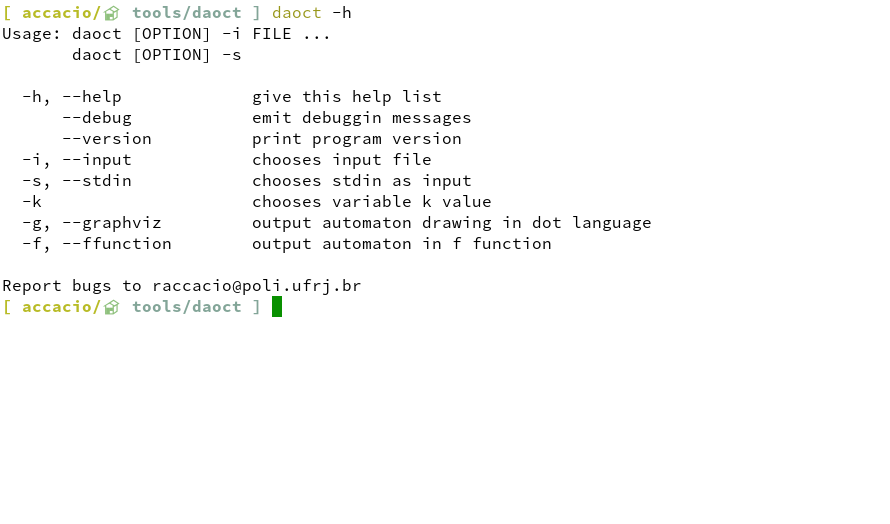
\includegraphics[trim={0 7cm 0cm
    0},clip,width=\textwidth]{tools/daoct/daoctHelp.png}
  \caption{daoct help dialog.}
  \label{fig:daoctHelp}
\end{figure}

An example of a csv input and the script's different outputs can
be seen in the following figures:
\vspace{-1cm}
\begin{figure}[H]
\begin{minipage}[H]{0.5\textwidth}
  \centering 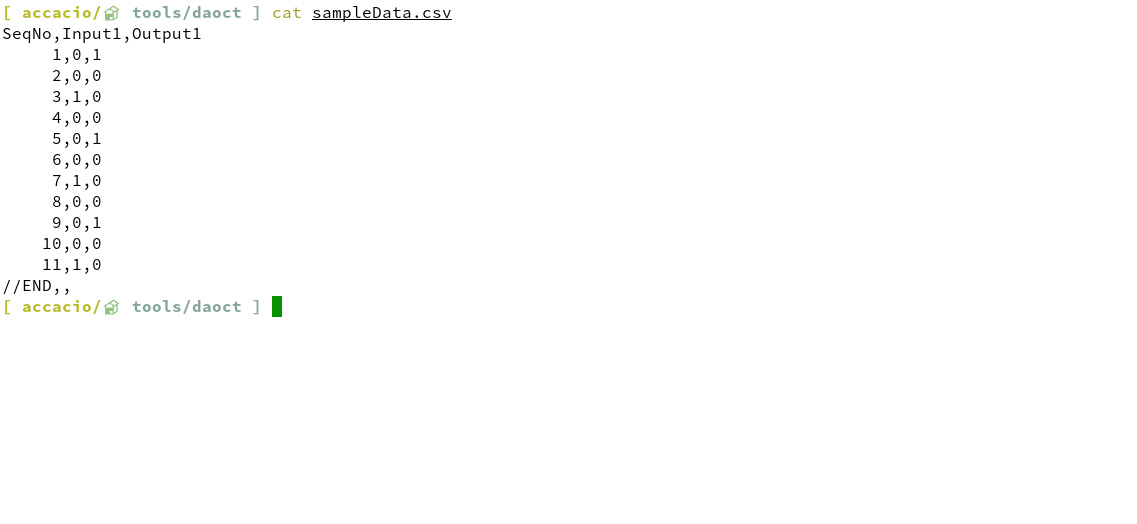
\includegraphics[trim={0 4cm 24cm
    0},clip,width=0.9\textwidth]{tools/daoct/daoctInput.png}
  \caption{daoct csv input file.}
  \label{fig:daoctInput}
\end{minipage}
\begin{minipage}[H]{0.5\textwidth}
  \centering 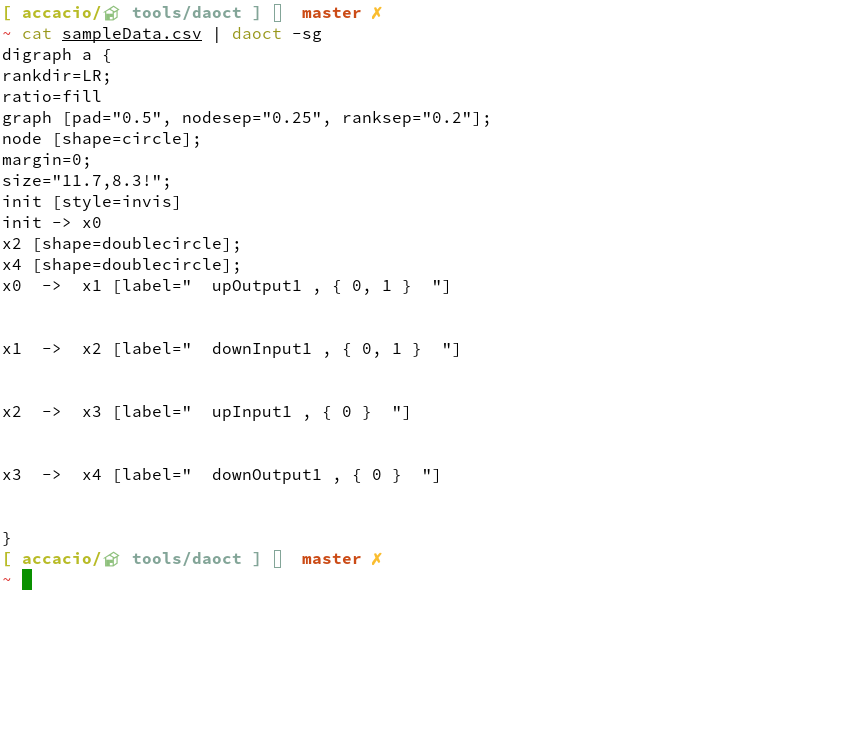
\includegraphics[trim={0 3cm 15cm
    0},clip,width=1.2\textwidth]{tools/daoct/daoctOutput.png}
  \caption{daoct graphviz output.}
  \label{fig:daoctOutput}
\end{minipage}
\end{figure}  


\begin{figure}[H]
  \centering
  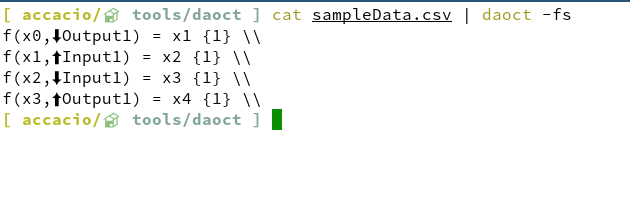
\includegraphics[trim={0 2cm 2cm
    0.1cm},clip,width=0.6\textwidth]{tools/daoct/daoctOutputFfunction.png}
  \caption{daoct \ffunction{} function output.}
  \label{fig:daoctOutputFfunction}
\end{figure}

% \lstinputlisting[caption=daoct
% main,language=Python]{../../tools/python/DAOCT/daoct}

% \definecolor{keywordstyle}{rgb}{0,1,0.82} \lstinputlisting[caption=daoct
% ,language=Python]{../../tools/python/DAOCT/daoct.py}

% \lstinputlisting[caption=Utils
% ,language=Python]{../../tools/python/DAOCT/utils.py}

% \lstinputlisting[caption=Automaton
% ,language=Python]{../../tools/python/DAOCT/automaton.py}

\section{dot2automata}
\label{sec:dot2automata}

To visualize the output of the daoct program, the script \verb|dot2automata| was
created. It's basically a wrapper of the \verb|dot2tex| program, that is capable of
transforming a dot file in a tex file with the tikz syntax. \verb|dot2automata|
pre-process the dot file so the tikz output can be drawn using automaton style,
with states and marked states, similar to graphs used in \cite{moreira2018enhanced}.
An example of the output of the help option can be seen in \autoref{fig:dot2automataHelp}
\tikzset{every node/.style={align=center}}

\begin{figure}[H]
  \centering
  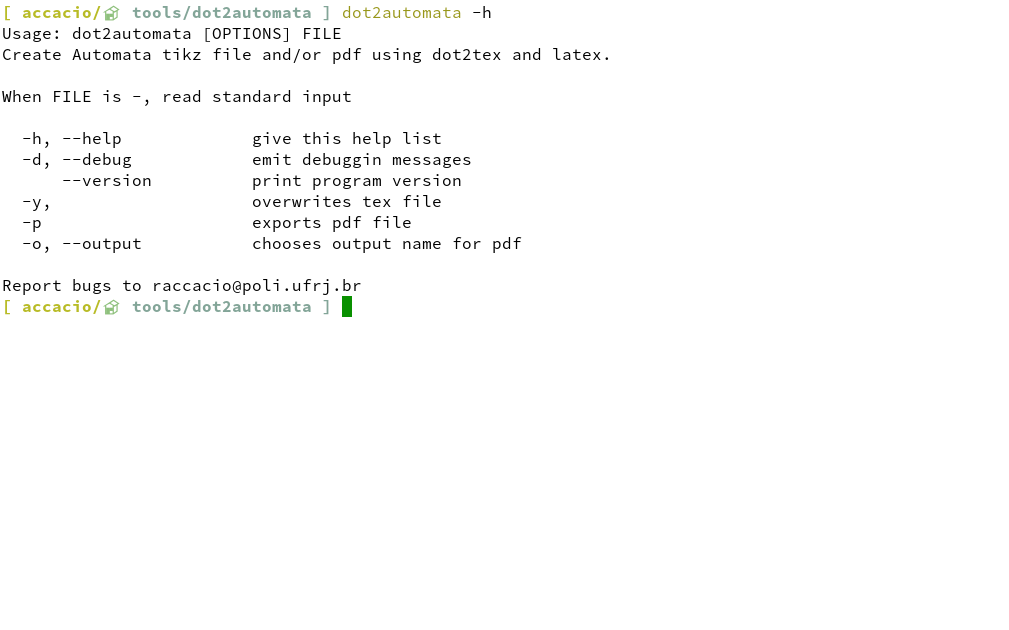
\includegraphics[trim={0 10cm 5cm
    0},clip,width=\textwidth]{tools/dot2automata/dot2automataHelp.png}
  \caption{dot2automata Help.}
  \label{fig:dot2automataHelp}
\end{figure}

As we can see there is an option to output a pdf file, so we can have a preview
of the image. The tikz figure can be included in a latex and resized using the
tikzscale package. So including a file as in \autoref{lst:Includetikz} can
result in the \autoref{fig:Dot2automataSampleOutput}

\lstset{%
  % basicstyle=\small\ttfamily,
  language=[LaTeX]{TeX}
}
\begin{lstlisting}[caption=Include tikz file.,label={lst:Includetikz},numbers=none]
\begin{figure}[H]
  \centering
  \includegraphics[width=\textwidth]{tools/dot2automata/sampleData.tikz}
  \caption{dot2automata output.}
\end{figure}
\end{lstlisting}
\begin{figure}[H]
  \centering
  \includegraphics[width=\textwidth]{tools/dot2automata/sampleData.tikz}
  \caption{dot2automata output.}
  \label{fig:Dot2automataSampleOutput}
\end{figure}


% \lstinputlisting[caption=configPetriNet,language=bash]{../../tools/bash/configPetriNet}

% \lstinputlisting[caption=dot2automata,language=bash]{../../tools/bash/dot2automata}

% \lstinputlisting[caption=dot2petri,language=bash]{../../tools/bash/dot2petri}

% \lstinputlisting[caption=linkPetriNets,language=bash]{../../tools/bash/linkPetriNets}

% \lstinputlisting[caption=linkTables,language=bash]{../../tools/bash/linkTables}

% \lstinputlisting[caption=petriml2dot,language=bash]{../../tools/bash/petriml2dot}

% \lstinputlisting[caption=removeVarsFromData,language=bash]{../../tools/bash/removeVarsFromData}

% \lstinputlisting[caption=treatCSV,language=bash]{../../tools/bash/treatCSV}

\section{dot2petri}
\label{sec:dot2petri}

The script \verb|dot2petri| is a similar to \verb|dot2automata|, the same
working principle but a different objective, this time the objective is to
visualize Petri Nets. It's help dialog it's almost the same of dot2automata:
\begin{figure}[H]
  \centering
  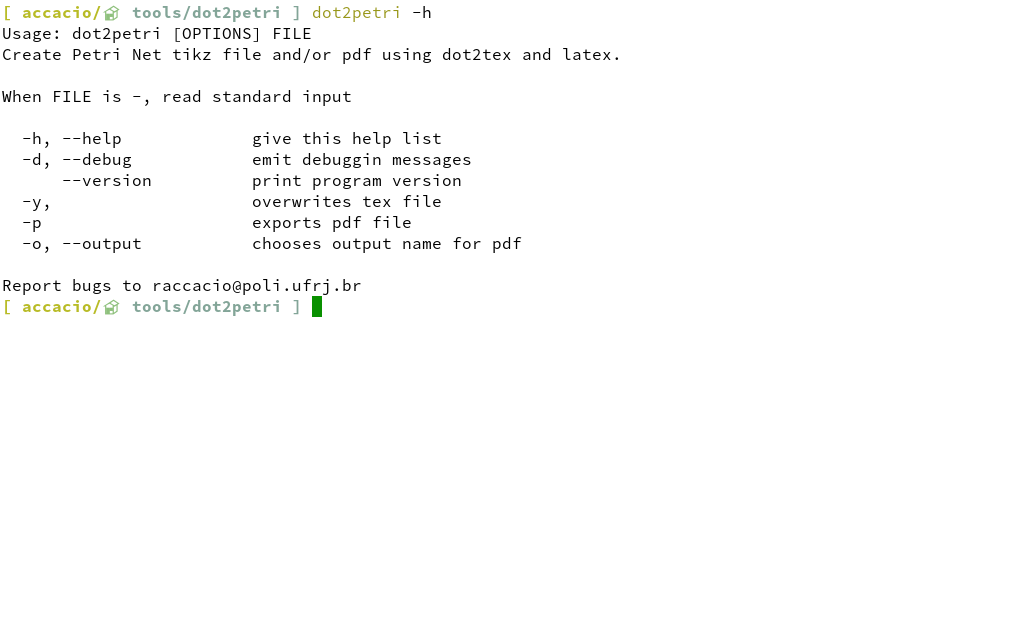
\includegraphics[trim={0 10cm 5cm
    0},clip,width=\textwidth]{tools/dot2petri/dot2petriHelp.png}
  \caption{dot2petri Help.}
  \label{fig:dot2petriHelp}
\end{figure}

The input dot file has a syntax slightly different from `plain vanilla' dot
language, as we can see in the following listing:

\lstinputlisting[caption={dot2petri input dot
  file.},label={lst:dot2petriSampleData},numbers=none,basicstyle=\scriptsize]{../../figures/tools/dot2petri/sampleData.dot}

Using this modified syntax it is easy to define places, marked places,
transitions, timed transitions, and different kinds of arcs. Places are defined
using `p' followed by an identification number, marked places are similar to
places but have the letter `m' and a number appended, this number represents how
many tokens are in this place. Transitions are defined with a simple `t'
followed by its identification number and timed transitions are created using `tt' and the
id. The arcs can be defined using `->' between two tags (between places and
transitions), an inhibitor arc can be created changing the style of the arc, and
a label can be used to define the number of tokens that are needed to trigger
the transition or the number of tokens inserted in a place. A tikz style for places
and transitions that are external to the current Petri Net are drawn using
dotted lines, so we can see where different parts interconnect themselves.

Such dot files can be created in two ways: manually writing them or using
another script called \verb|petriml2dot| present in the same repository. This
other script converts a file in petriml, created using the Platform Independent Petri
net Editor 2 (PIPE2)\footnote{\url{http://pipe2.sourceforge.net/}} to the dot
format.
PIPE2 is a very powerful tool to design Petri Nets, since it is possible to simulate the
net and it can generate reachability graphs, but at its current version, it lacks of a
good way to export the graph besides eps non-vector graphic, enter the \verb|petriml2dot| and \verb|dot2petri| scripts.

The code shown in \Autoref{lst:dot2petriSampleData} used as input for the
\verb|dot2petri| script outputs a tikz file, that included in a similar fashion
to the one shown in \Autoref{lst:Includetikz}, can result in the following figure:

\begin{figure}[H]
  \centering
  \includegraphics[width=0.9\textwidth]{tools/dot2petri/sampleData.tikz}
  \caption{dot2petri output.}
  \label{fig:Dot2automataSampleOutput}
\end{figure}

\section{Other Scripts}
\label{sec:otherScripts}
A couple of other scripts were created to ease the building process. The 
\verb|linkPetriNets| and \verb|linkTables|, for instance, that together can link tex tables to
tikz petri net figures, so they can hyperlinked in digital format, as seen in
\Autoref{fig:petriInitialization}. And other scripts that can pre-process the csv
tables before sending to \verb|daoct|, as in \verb|treatCSV| and \verb|removeVarsFromData|.


%%% Local Variables:
%%% mode: latex
%%% TeX-master: "../monografia"
%%% End:
